\section{Self-confidence Factorization and Calculation} \label{sec:self-confidence}
    \begin{figure}[tbp]
        \centering
        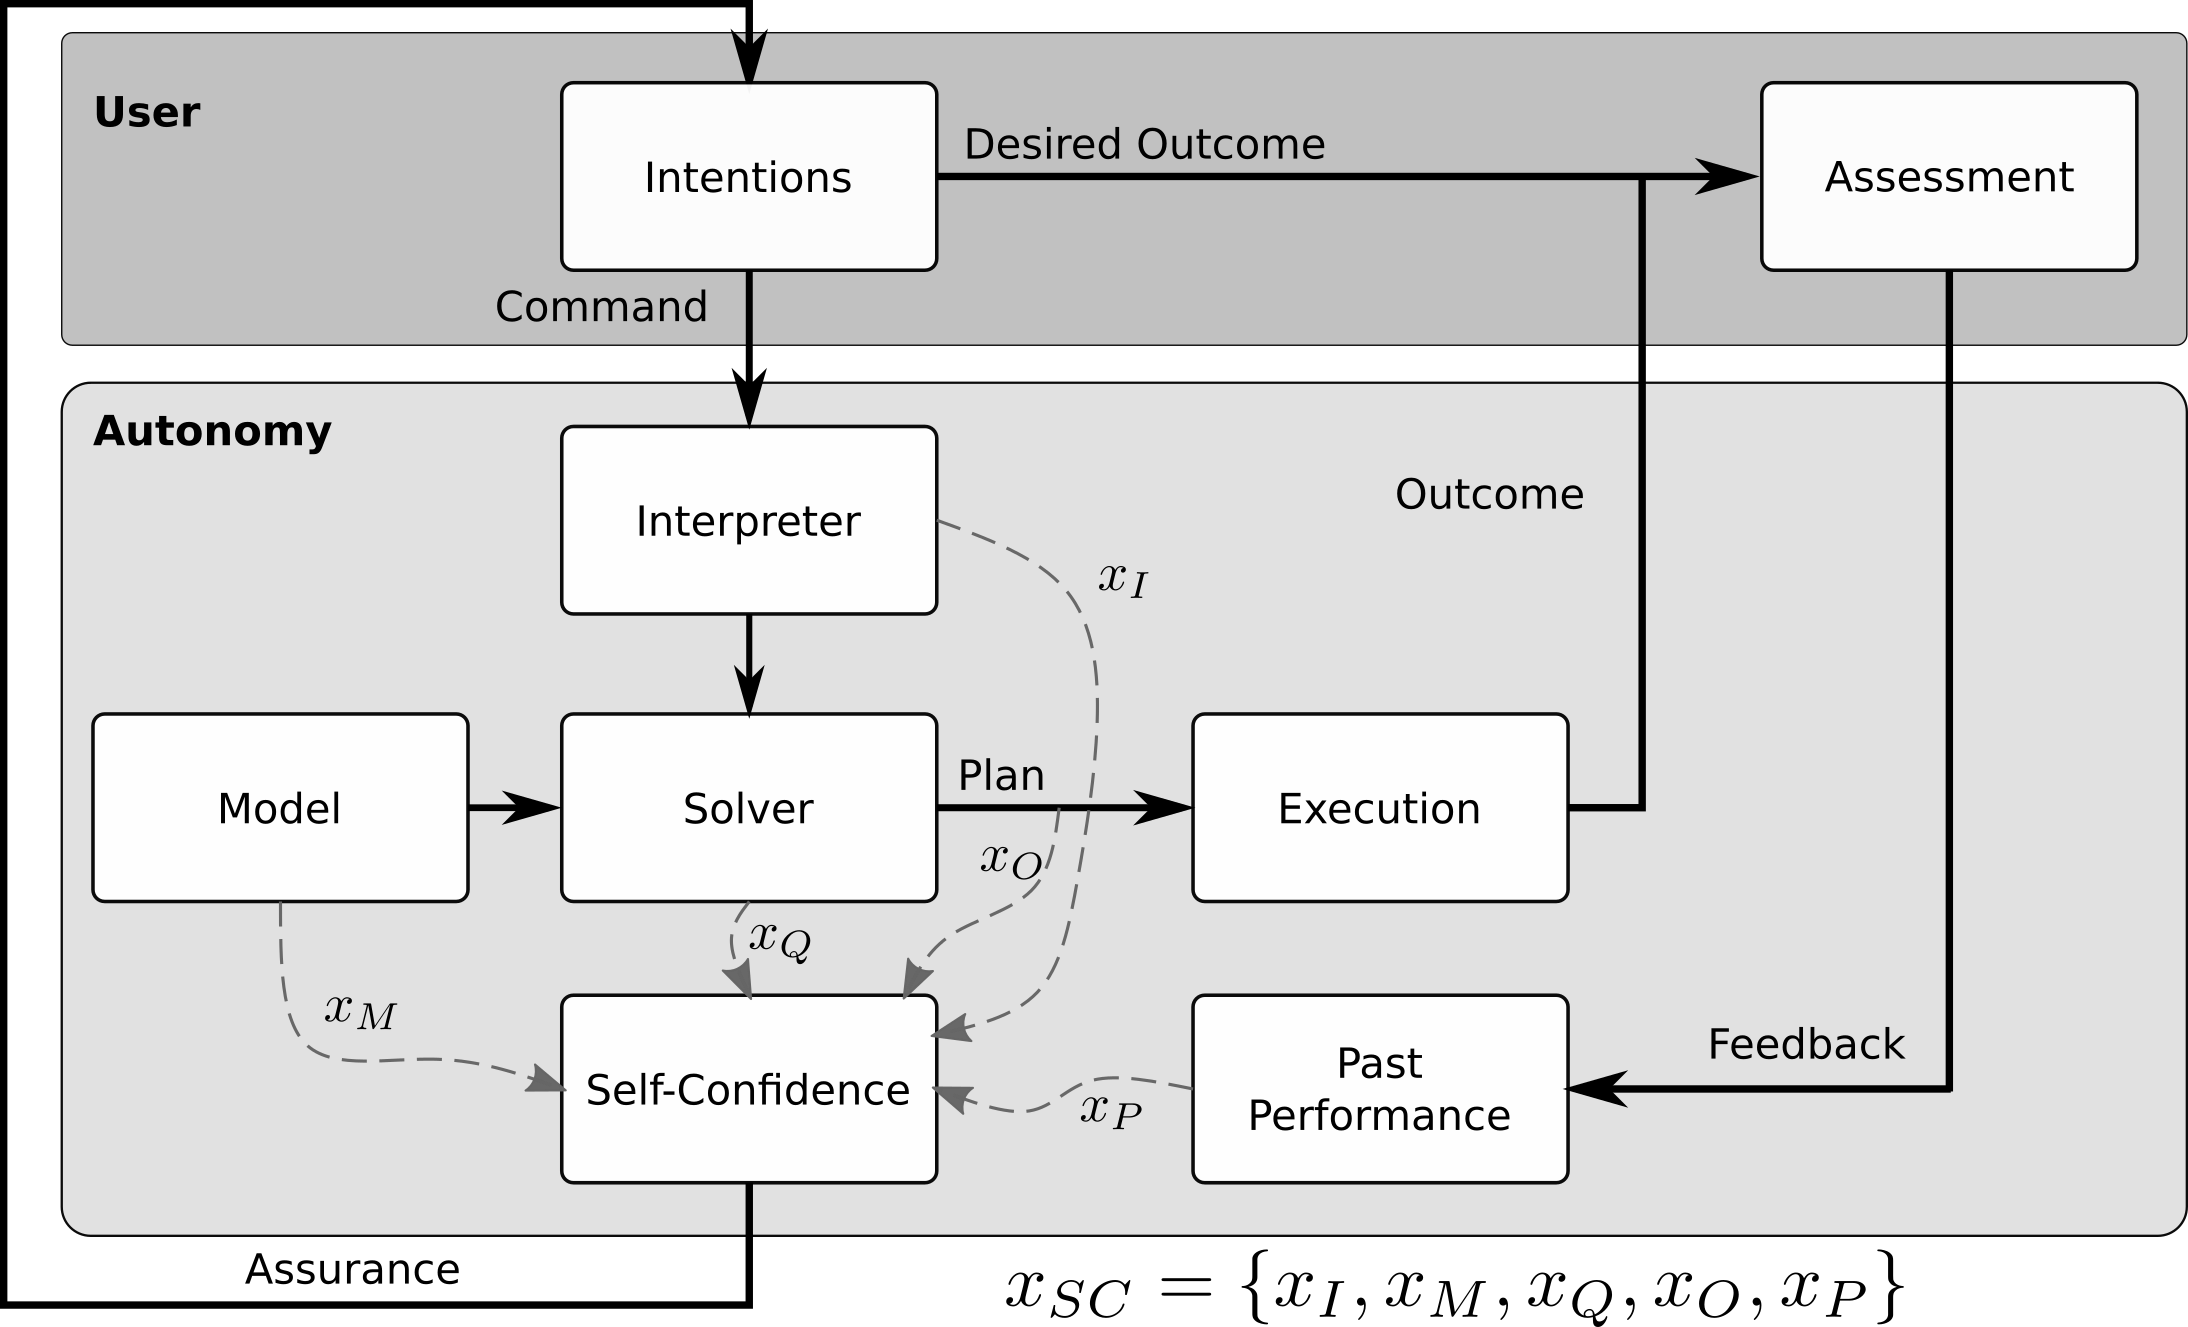
\includegraphics[width=0.90\linewidth]{Figures/FaMSeC.png}
        \caption{Factorized Machine Self-Confidence (\famsec)}
        \label{fig:famsec}
    \end{figure}
    
    This work seeks to develop algorithmic strategies for assessing and communicating machine self-confidence. Of particular interest are model-based techniques that endow an APS with a process-driven scoring of how it arrives at decisions, and what factors influence the quality of its reasoning, in order to quantitatively assess its own competency boundaries. As such, it is important to formally establish both: (i) a set of principles, definitions, and relations that govern the `arithmetic of machine self-confidence' as a function of task, environment, system realization, and context, and (ii) variables, representations and operations for producing meaningful self-confidence assessments. 
    
    We initially address these issues for APS that are primarily defined by capabilities for dynamic decision-making and planning under uncertainty. This approach provides a pathway to developing firm initial mathematical and computational bases for addressing (i) and (ii) via the rich set of analytical and computational features inherent to the MDP model family. Insights developed along these lines can provide the basis of future work for formulating self-confidence computation strategies, other important planning model families, and APS capabilities that are formally related to decision making under uncertainty, such as dynamic learning and partially observable planning with sensing and perception. 
    After reviewing a computational framework for self-confidence assessment that relies on assessing individual factors involved with solving MDP-based planning and decision-making problems, we consider how one of these factors (related to the quality of a given MDP policy solver) can actually be computed, building on insights derived from calculation and analysis of another factor (related to intrinsic task difficulty) examined in other work. 
    
    \subsection{The \famsec{} Framework }
    The approach presented here adopts and builds on the \emph{Factorized Machine Self-Confidence (\famsec)} framework developed in ref. \cite{Aitken2016-cv, Aitken2016-fb}. The key idea behind \famsec{} is to represent and compute self-confidence as a traceable multi-factor function, which combines shorthand assessments of where and when operations and approximations inherent to model-based autonomous decision-making are expected to break down. As with the self-confidence reporting strategy developed in \cite{Hutchins2015-if}, this captures metrics than an expert designer would use to assess the correctness and quality of an autonomous decision-making system, accounting for variations in task, environment, system implementation, and context. However, unlike \cite{Hutchins2015-if}, \famsec{} allows an APS to automatically generate its own holistic assessments of self-confidence, i.e. without the need for a human designer/expert to specify a priori how self-confident a system ought to be given such variations %%(which can be cumbersome, if not impossible, to fully account for in practical applications). 
    
    Figure \ref{fig:famsec} illustrates \famsec's notional overall self-confidence scoring mechanism. This uses a distinct set of \emph{self-confidence factors} (dashed lines) that are derived from core algorithmic decision-making components (white boxes in the `Autonomy' block). The total self-confidence score can be mapped onto an arbitrary scale, e.g. -1 to +1 for the sake of discussion, where -1 gives a shorthand indication of `complete lack of confidence' (i.e. some aspect of task, environment, or context falls completely outside the system's competency boundaries), and +1 indicates `complete confidence' (i.e. all aspects of task, environment, and mission context are well within system's competency boundaries). As will be shown later, the scales for each factor need not all be the same and can carry slightly different qualitative interpretations, as long as a clear sense of `confidence direction' (i.e. degree of self-trust) can be established for each. 
    Ref. \cite{Aitken2016-cv} considers five general factors that contribute to a `total self-confidence score', which notionally maps the multivariate the combined set of individual factors into an overall confidence report:
    
    
\begin{enumerate}
\item \xI---\textit{\textbf{interpretation of user intent and task}}: To what extent were the user's intentions properly understood and translated by the autonomous system into context-appropriate mission specifications and tasks? This factor derives from features and parameters of the `Interpreter' block. For instance, if a natural language interface is used for mission planning, this factor could assess how well user inputs are mapped to reward functions using fixed vocabularies for different mission profiles. 
%This factor can, for instance, capture uncertainty in task objectives or reward functions \cite{abbeel2004apprenticeship, hadfield2016cooperative}. 
%
\item \xM---\textit{\textbf{model and data validity}}: Are the agent's learned and/or assumed models, and associated training data used for decision-making good enough proxies for the real world? This factor assesses how well the set of measurements and events predicted by the autonomous system line up with what it actually should observe in reality. 

%Specifically, this factor uses features and parameters of the `Model' block to assess how well the set of measurements and events predicted by the autonomous system line up with what it actually should observe in reality. 
%For the U2R2 problem, model validity is related to the size of the state space of the model and the level of discretization used in the environment and action set.
%
\item \xQ---\textit{\textbf{solver quality}}: Are the approximations and learning-based adaptations used by the system for solving decision-making problems appropriate for the given mission and model? 
%%This factor uses features and parameters of the `Solver' block to assess the ability of the system to make appropriate decisions based on the information it is given. This factor directly assesses a key aspect of the inherent fitness of the reasoning process: s
Since approximations are almost always needed to solve otherwise intractable decision making problems, this factor examines the appropriateness and reliability of those approximations. 
%For instance, if it is too costly to implement optimal planning, certain problem constraints can often be relaxed to arrive at nearly optimal decisions more cheaply; if such approximations are invalid in critical portions of the problem space, then these can result in poor decisions and hence low confidence in the solution quality. 
This factor also accounts for the impact of learning mechanisms required to make complex decisions under uncertainty, e.g. based on suitability of training data or the learning process to solving the problem at hand. 
%%\nraComm{Ufuk: here is the hook to talk about assessment of learning in MDP families...}
%For the U2R2 problem we will use a priori bounds on the optimality of the resulting policy given known properties of the model and data.
%
\item \xO---\textit{\textbf{expected outcome assessment}}: Do the sets of possible events, rewards, costs, utilities, etc. for a particular decision lead to desirable outcomes? 
Even if the autonomous system perfectly understands and analyzes a task, and can arrive at globally optimal solutions, it may still not be able to always avoid running into undesirable states along the way. % (e.g. due to the existence of catastrophic events with small but non-zero probabilities). 
This factor evaluates the particular decision making strategy implemented by the system to assess the inherent favorability of the full landscape of possible task outcomes.  
%For stochastic policies we use a variation of the upside potential ratio to assess the expected outcome. This measure is further weighted to account for known human biases at extreme outcome probabilities [XYZ]. 
%
\item \xP---\textit{\textbf{past history and experiences}}: What can be gleaned from the system's own experience and other available historical information for past problem instances?  
This factor notionally allows the autonomous system to predict, transfer, and update assessments of self-confidence based on prior experiences, and thus embodies meta-memory and meta-learning for enabling and improving self-assessments. 
%For the U2R2 problem we use a combination of the current learned policy and the rate of change of the policy around the current state to determine how past performance should correlate with current behavior. 
\end{enumerate}

Since the overall self-confidence mapping is heavily dependent on application, context, and desired levels/types of user-autonomy interaction, this work assumes for simplicity that the overall mapping consists of a direct report of some fixed subset of the component factors, i.e. \xSC. 
Furthermore, the five factors considered here are neither exclusive nor exhaustive. For example, the factors developed by \cite{Aitken2016-cv, Aitken2016-fb} are primarily aimed at self-assessment \emph{prior} to the execution of a particular task, whereas it is conceivable that other self-confidence factors could be included to account for in situ and post hoc self-assessments. For simplicity, attention is restricted to the a priori task self-assessment case. \nisar{where is traceability mentioned?  notional ability for user to `drill down'?}
%%Incidentally, these characteristics of self-confidence (i.e. self-trust) component factors are not dissimilar from the multidimensional and contextual nature of the component factors that comprise human trust. 

%\nisar{edit...} Self-confidence \xSC{} is a composite assurance \nisar{do we need more jargon?} that stems from some combination of these five factors. 

\subsubsection{VIP Escort Example Revisited}

We will use the VIP Escort scenario to examine two immediate questions: (i) how should the factors be expected to behave under different conditions (independently of how they are actually calculated)?, and (ii) how should any one these factors actually be calculated?  

To address (i), we should first consider what kinds of trends, `boundary conditions', and interactions are expected for the various factors if we are given some class of solver for the underlying UGV motion planning problem. For instance, if the problem were modeled and encoded as a discrete-time/discrete-space POMDP, then sampling-based Monte Carlo solvers could be used to find an approximately optimal policy $\pi$ \cite{Silver-NIPS-2010, Thrun-ProbRobotics-2006}\brett{fix this!}, which would map Bayesian beliefs about the chaser state given the UGS data onto specific UGV actions to maximize the UGV's expected cumulative reward. Figure \ref{fig:trendsBCs} shows some expected behaviors for the \famsec{} factors for such a solver, as a function of task, environment, system, and context, assuming again an arbitrary finite range of -1 (total lack of confidence) to +1 (complete confidence) for illustration only. For instance, \xQ{} would logically be expected to increase/decrease as the number of samples used by the Monte Carlo solver to approximate $\pi$ increased/decreased. Similar trends could also be derived for other non-sampling based solvers. \nisar{mention about traceability/drill down basis here?}

With this in mind, an important issue to consider for addressing (ii) is that the factors can depend on each other in complex ways. A logical simplifying assumption for initial algorithm development is thus to consider cases where we can ignore the interactions between factors; this is equivalent to examining each factor along `boundary conditions' where other factors do not change and thus have little/no contribution to the overall self-confidence score. For example, ref. \cite{Aitken2016-cv} developed an approach to compute \xO{} for infinite horizon MDP and POMDP planning, assuming the boundary conditions \xM$=+1$ (perfectly known problem/task model), \xI $= +1$ (perfectly interpreted user task command and reward function $R_k$), \xQ$=+1$ (optimal policy $\pi$ known and available), and \xP$=+1$ (task encountered previously). Under these conditions, overall self-confidence depends only on \xO, which can then be quantified as a measure of the probability distribution $p_{\pi}(R_{\infty})$ of achievable cumulative reward values $R_{\infty} = \sum_{k=0}^{\infty}R_{k}$ under policy $\pi$. Ref. \cite{Aitken2016-cv} considers several measures of $p_{\pi}(R_{\infty})$, including the logistically transformed upper partial moment/lower partial moment (UPM/LPM) score, which quantifies how much probability mass lies to the right vs. left of a minimally acceptable cumulative reward value $R^*_{\infty}$ (e.g. in the basic VIP Escort problem, this corresponds to a user-specified maximum acceptable time to successfully reach the exit).

By indicating how likely favorable outcomes are expected relative to unfavorable outcomes according to a baseline performance measure $R^*_{\infty}$, self-confidence measures like the UPM/LPM score provides information about the consequences of applying policy $\pi$ to a task by interpreting the full shape of the cumulative reward distribution $p_{\pi}(R_{\infty})$, i.e. beyond just the mean value of $R_{\infty}$ (which the optimal $\pi$ maximizes) or the variance/entropy of $p_{\pi}(R_{\infty})$. As illustrated in Fig.~\ref{fig:xOexample} this allows \xO{} to be used as a second-order uncertainty measure for assessing intrinsic task difficulty---and hence indicates a measure of APS competency that can be used to calibrate user trust. \nisar{explanations underneath figs not obvious -- mention how user could drill?}

\nisar{How to extend insights to computing other s/c factors? -- in particular, work by Aitken in \cite{Aitken2016-cv} did not specify how to compute other factors, nor how to cope with interdependencies between factors that will arise when assumptions such as those above are relaxed? From famsec block diagram fig, one approach is to work backwards from \xO, and examine how similar kinds of information can inform different factor calculations under different/related/progressively relaxed boundary conditions ... in particular, since \xO indirectly depends on \xQ per famsec block diagram, we consider how to use $p(R_{\infty})$ to also derive a metric for \xQ ... namely, if we consider that an MDP-/POMDP-based APS must in practice often rely on an approximate policy $\tilde{\pi}$ instead of the true optimal policy $\pi$, then a quantitative comparison of $p_{\tilde{\pi}}(R_{\infty})$ to $p_{\pi}(R_{\infty})$ provides a metric for \xQ...the remainder of this paper explores how strategies for actually calculating/assessing \xQ along these lines... }

%Ref. \cite{Aitken2016-cv} considers several measures of $p_{\pi}(R_{\infty})$, such as the logistically transformed upper partial moment/lower partial moment (UPM/LPM) score, which quantifies how much probability mass lies to the right vs. left of a minimally acceptable cumulative reward value $R^*_{\infty}$ (e.g. in the basic VIP Escort problem, this corresponds to a user-specified maximum acceptable time to successfully reach the exit). By indicating how likely favorable outcomes are expected relative to unfavorable outcomes according to a baseline performance measure $R^*_{\infty}$, self-confidence measures like the UPM/LPM score provides information about the consequences of applying policy $\pi$ to a task by interpreting the full shape of the cumulative reward distribution $p_{\pi}(R_{\infty})$, i.e. beyond just the mean value of $R_{\infty}$ (which the optimal $\pi$ maximizes) or the variance/entropy of $p_{\pi}(R_{\infty})$. This allows \xO{} to be used a second-order uncertainty measure for assessing intrinsic task difficulty -- and hence indicates a measure of APS competency that can be used to calibrate user trust. \nisar{would including a simple graphical example from Matt's thesis in next section help?}
%%\xO{} was been previously defined in \cite{Aitken2016-cv}, but has not yet been evaluated as an effective assurance as per the guidelines laid out in the work on assurances. Herein \xQ{} is investigated. 

\begin{figure}[tbp]
    \centering
    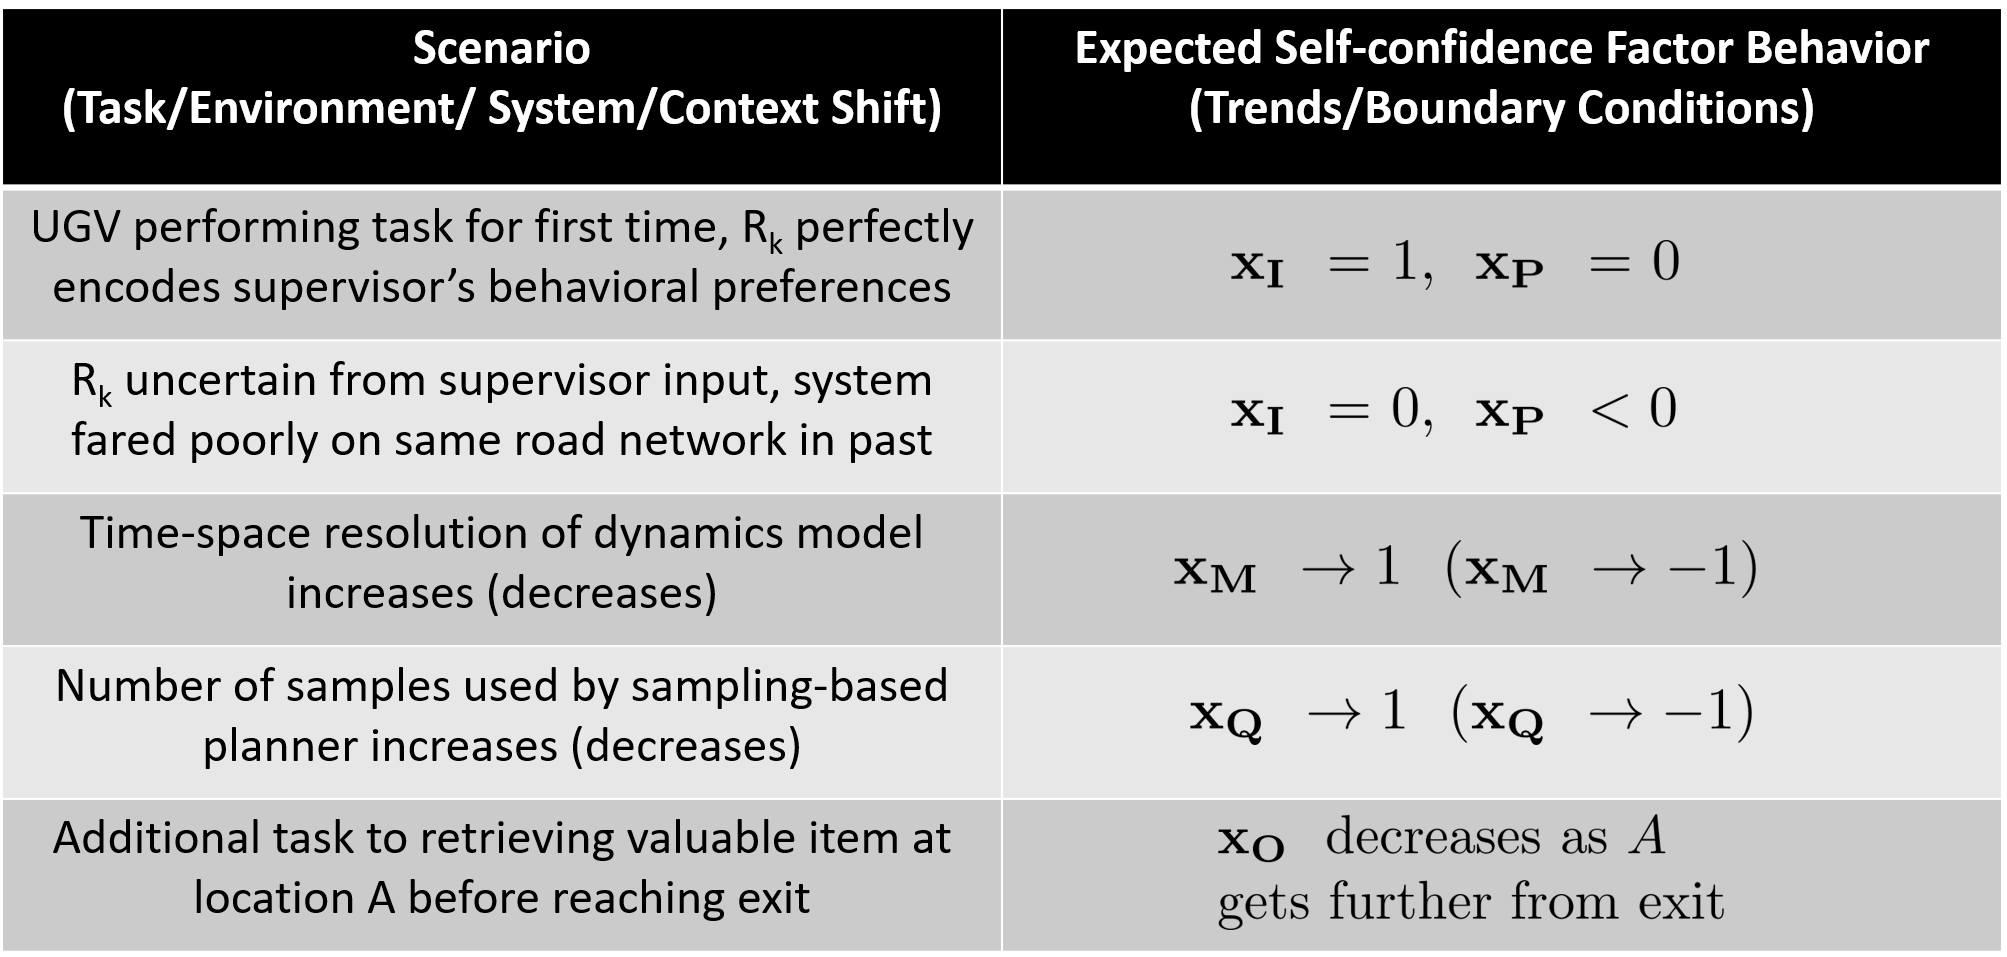
\includegraphics[width=0.99\linewidth]{Figures/scTrendsBoundaryExample.png}
    \caption{Notional \famsec{} behaviors for VIP Escort problem with a hypothetical sampling-based solver.}
    \label{fig:trendsBCs}
%    \vspace{-0.3 in}
\end{figure}

\begin{figure}[tbp]
    \centering
    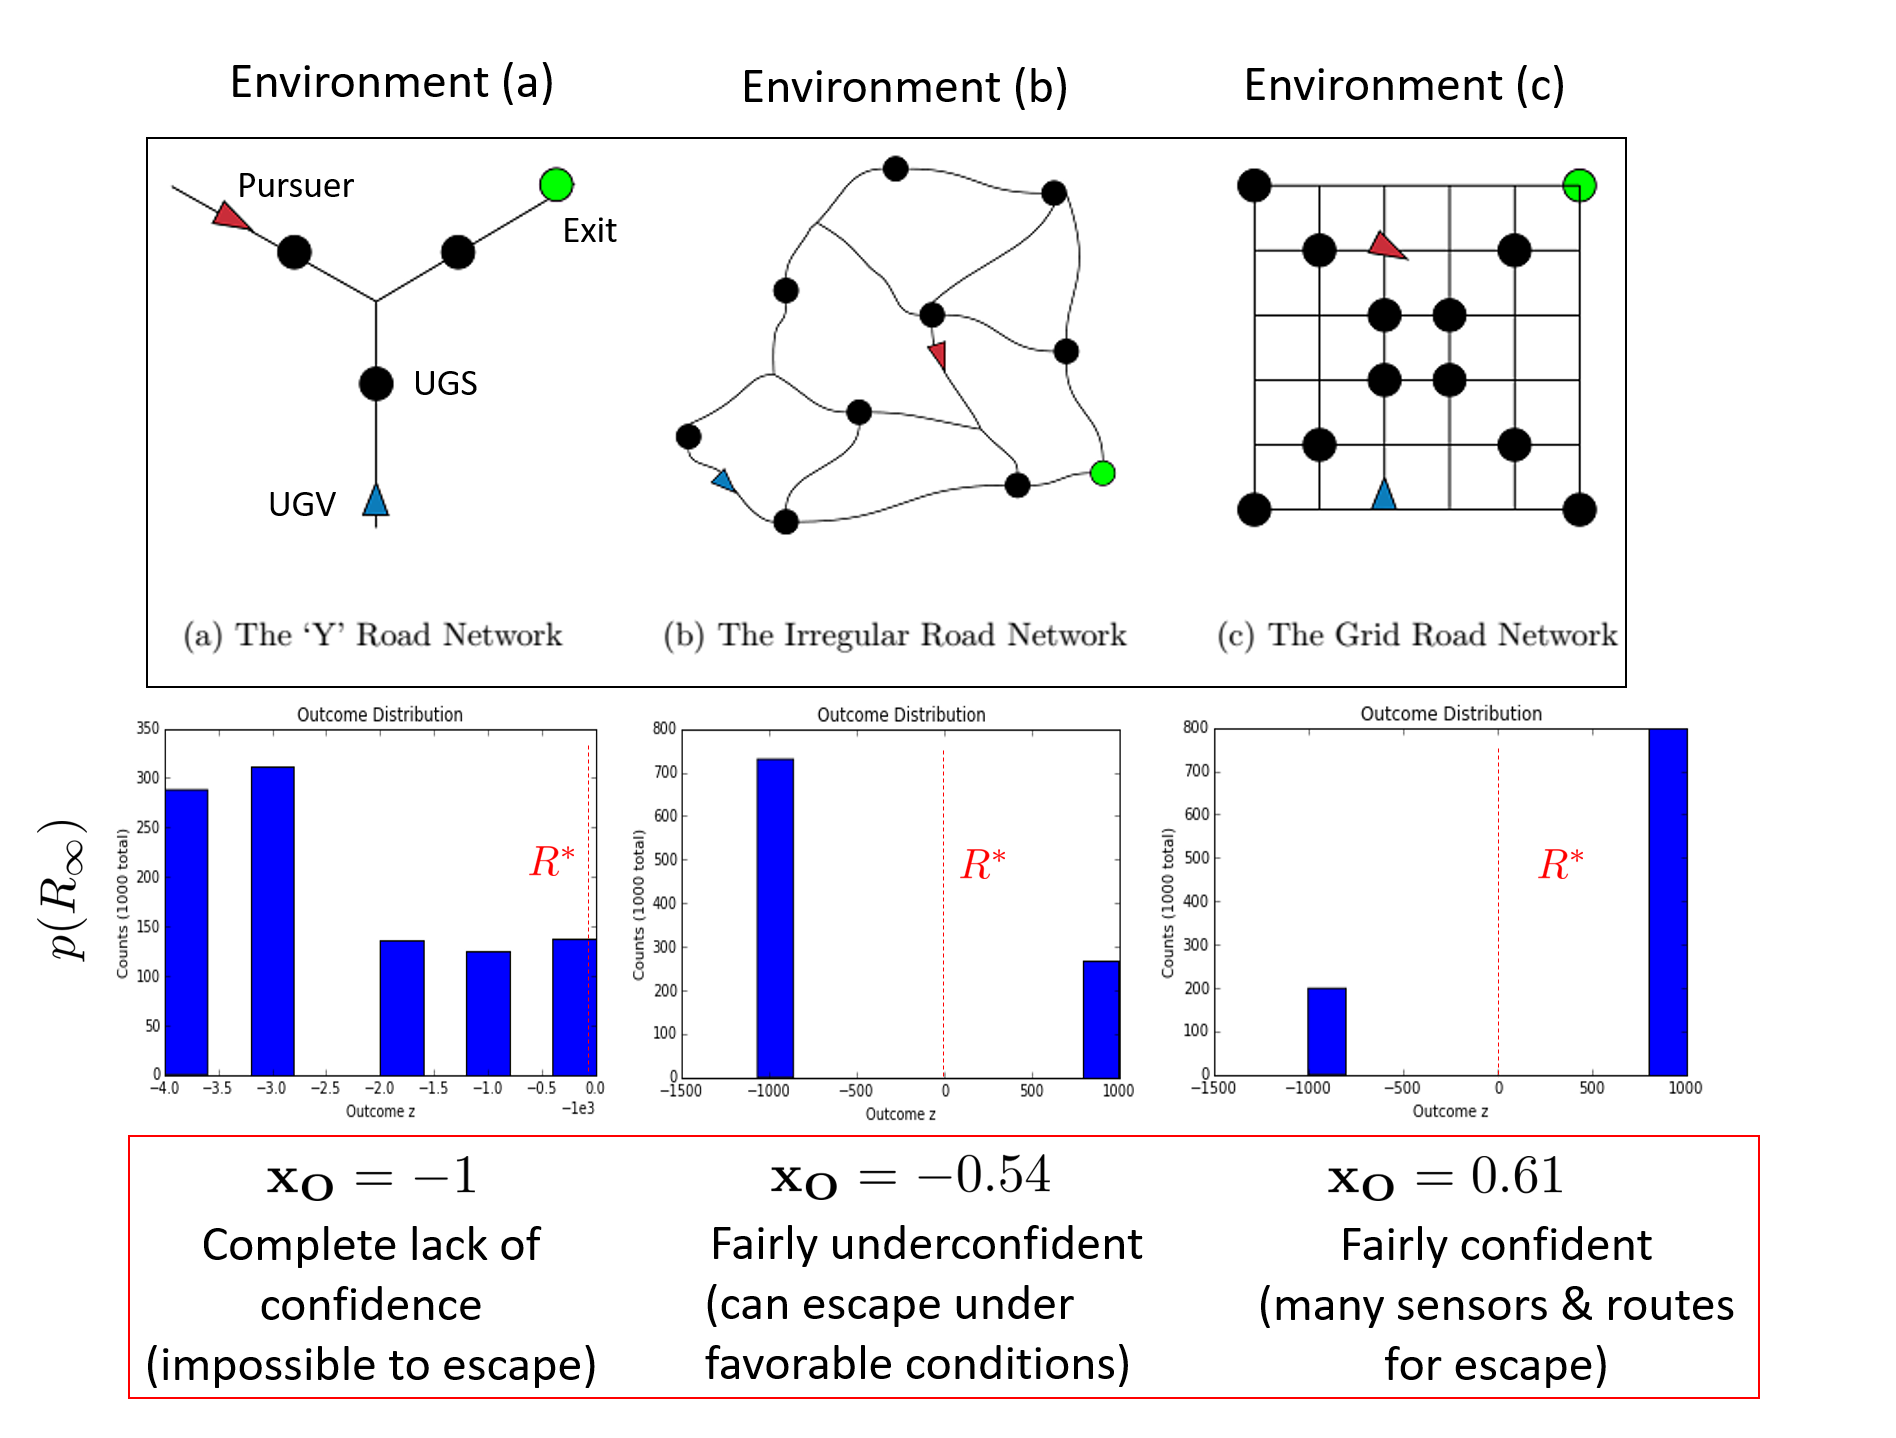
\includegraphics[width=0.99\linewidth]{Figures/xO_envsOnly.png}
    \caption{Example \xO{} assessments for VIP Escort problem in various task environments, using UPM/LPM score from \cite{Aitken2016-cv} on empirically sampled $p(R_{\infty})$ pdfs.}
    \label{fig:xOexample}
%    \vspace{-0.3 in}
\end{figure}


\subsection{Solver Quality (\xQ)} \label{sec:SQ}
    The main aim of \xQ{} is to indicate how a solver \solve{} will perform on a given (possibly un-encountered) task \task{} of a given class \taskclass{} (i.e. all road networks with a UGV, Pursuer, and exit, et cetera as described previously). The need for \xQ{} is not necessarily easy to understand; an analogy helps to clarify:
    
    \emph{Clarifying Example:} Think of \xQ{} as an indication of the \emph{ability} of an athlete. This is opposed to the athlete's assessment of the desirability of the outcome of a game (\xO). While an athlete may be very capable (high \xQ), the score of the game may be such that the athlete knows that it is nearly impossible to catch up and win the game (low \xO). Conversely, an athlete may not be very capable (low \xQ), and due to being na\"{i}ve has an incorrect assessment of the desirability of the outcome (\xO{} cannot be trusted).
    
    The formal desiderata for \xQ{} are:
    
    \begin{enumerate}[label=\textbf{D\arabic*}]
        \item reflect competence of solver \solve{} for task \task{} (where competence is analogous to the `ability' of the athlete in the example)\label{itm:d1}
        \item enable comparison across solver classes \label{itm:d2}
        \item extend to unseen tasks of the same class \taskclass \label{itm:d3}
    \end{enumerate}
    
    For practical application, it is critical to be able to compare the quality of solvers of different classes (i.e. exact vs. approximate) because there are many different ways of solving tasks. Likewise, it is also common for an APS to encounter a similar, but previously unseen, task (i.e. a different road network).
    
    Evaluating the `quality' of something implies some kind of comparison is taking place. In this setting the desired comparison is between a `candidate solver' \solve{} and some reference solver. Ideally, the candidate solver could be compared to the exact solution (whose quality is by definition perfect), but there are three main challenges:

    \begin{enumerate}[label=\textbf{C\arabic*}]
        \item It is unclear how policies/solvers should be compared \label{itm:l1}
        \item Large state spaces make exact solutions infeasible \label{itm:l2}
        \item It is generally impossible to evaluate the exact solution for \emph{all} tasks of a given task class \taskclass{} (linked to \ref{itm:d3}) \label{itm:l3}
    \end{enumerate}

    \subsubsection{Addressing \ref{itm:l1}} \label{sec:compare_policies}
        Solvers of all classes are similar in that they operate on a specified problem in order to produce a policy $\pi$ that is a mapping from states to actions with the aim of maximizing expected reward. A few possibilities for comparing policies include:
    
        \begin{enumerate}
            \item Compare utilities at each state \label{itm:i1}
            \begin{itemize}
                \item Merits: Evaluates whether states are assigned equal utility across solvers. Theoretically state utilities should be independent of the solver. Addresses \ref{itm:d1}
                \item Demerits: Doesn't address \ref{itm:d2}---Doesn't apply when different solvers represent different amounts of the state space, or represent the state space differently.
            \end{itemize} 
            \item Compare `coverage' of the policy (here coverage refers to the proportion of the total state space considered by the solver) \label{itm:i2}
            \begin{itemize}
                \item Merits: Evaluates how `thorough' the policy is; in concert with \ref{itm:i1} could address \ref{itm:d1}
                \item Demerits: Doesn't satisfy \ref{itm:d2}---not all policies have the same coverage, typically by design. Also, high coverage does not imply a `good' solution
            \end{itemize}
            \item Compare the reward distribution of given policies \label{itm:i3}
            \begin{itemize}
                \item Merits: Meets \ref{itm:d1}, also able to satisfy \ref{itm:d2} as reward distributions can be simulated from any policy
                \item Demerits: Expensive to calculate the reward distribution via many simulations
            \end{itemize}
        \end{enumerate}

        Of the possibilities listed above, item \ref{itm:i3} will be used because only it is able to satisfy \ref{itm:d1} and \ref{itm:d2}.

    \subsubsection{Addressing \ref{itm:l2}, and \ref{itm:l3}} \label{sec:practicality}
        In order to address \ref{itm:l2} a `trusted solver' \solvestar{} could be introduced as the reference to which the candidate solver \solve{} can be compared. This solver need not be exact (but could be). Ultimately, \solvestar{} is only required to be a reference of some kind; it may be optimal, or it may be abysmal. In fact given a space of all possible unseen tasks of class \taskclass, \solvestar{} will likely perform very poorly for some of them.

        Still, according to \ref{itm:l3}, it is impractical, or impossible, to find an exact solution for all tasks $\text{task class notation}$. Literature on `Empirical Hardness Models' (EHMs) lends some direction for confronting this challenge. In their work \cite{Leyton-Brown2009-yr,Hutter2009-og} introduced EHMs in order to predict the empirical runtime performance (as opposed to the `Big-O' runtime) of an algorithm on a problem with given features. Specifically, they investigate how the actual runtime of NP-complete problems can be predicted. Applying similar logic in the domain of APS, it should be possible to learn a surrogate model \surrogate{} that predicts the reward distribution \rwdstarapprox{} of a trusted solver \solvestar{} for a given task \task{} of class \taskclass. In this way it is possible to estimate the performance of \solvestar{} on problems to which it has never been applied. This approach also addresses \ref{itm:d3}.
        
    \subsubsection{Summary} The comparison of policies will be done through comparing reward distributions, and this approach addresses both \ref{itm:d1} and \ref{itm:d2}, along with \ref{itm:l1}. In order to address \ref{itm:l2} and \ref{itm:l3}, and \ref{itm:d3} a `trusted solver' \solvestar{} will be introduced to serve as a basis by which a `candidate solver' \solve{} can be evaluated. Furthermore a surrogate model \surrogate{} will be learned to predict \rwdstarapprox{} on un-encountered tasks. In this way, all desiderata, and challenges have been addressed.
        
   \begin{figure}[tb]
        \centering
        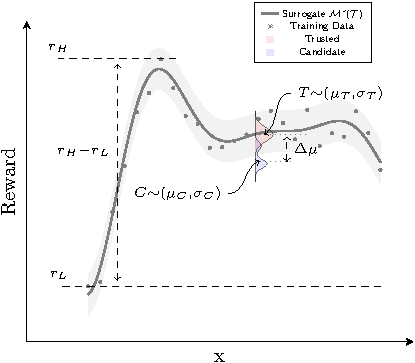
\includegraphics[width=0.75\linewidth]{Figures/sq_v2_fig-crop}
        \caption{Key values involved in calculating \xQ, where $x$ represents a `parameter of interest' for task \task, or solver \solve.}
        \label{fig:sq_v2}
    \end{figure}
